\documentclass{sigcomm-alternate}

\usepackage[utf8x]{inputenc}
\usepackage[hyphens]{url}
\usepackage{hyperref}

%\usepackage[longnamesfirst,sort,square]{natbib}


\begin{document} 
\title{Who Turned off the Internet?} 
\subtitle{Mining Temporary Unreachability\\ \Large Intermediate Report }

\numberofauthors{1} 
\author{ \alignauthor Daniel Aschwanden\\
%\affaddr{Communication Systems Group}\\
%\affaddr{Institute TIK}\\
\affaddr{ETH Zurich}\\
\email{asdaniel@ee.ethz.ch}\\
}

\maketitle 
%%%%%%%%%%%%%%%%%%%%%%%%%%%%%%%%%%%%%%%%%%%%%%%%%%%%%%%%%%%%%%%%
\section{Introduction}
% Problem: Connectivity problems exist
The end-to-end connectivity of hosts is the key service of the Internet. However, even after 40 years of intense engineering efforts, this connectivity is temporally broken for various reasons, such as link or hardware failure, mis-configurations, or natural disasters. 
% (Centrality Claim) Why do we care: Requires Troubleshooting Tools (TST) to minimize costs
This shows that there is a real need for methods to systematically detect and locate Internet outages of remote autonomous systems, subnets, and even single hosts. An automated, ongoing detection and tracking of connectivity issues of the Internet is particularly interesting for Internet Service Providers as it may generate transparent outage information for customers and enables the ISP to react adequately on a detected reachability problems and prevent expensive debugging sessions.

% (What is missing) Introduce the gap that we plan to close: 
Researches and industrial vendors have proposed various approaches for systematically detect, locate and troubleshoot Internet outages and loss of end-to-end reachability. % State clearly what is missing
A dominant share of researchers focussed on "pathological behavior related to the address space, e.g. bogon advertisements \cite{Feamster:2005}, prefix hijacking \cite{Zhang:2010}, BGP misconfigurations \cite{Mahajan:2002} or DDoS attacks \cite{Chen:2001}"\cite{Bush:Optometry}.

Basically, reachability can be viewed from two perspectives: data-plane and control-plane measurements. \cite{Bush:Optometry} pointed out that tracking data-plane reachability with control-plane information is heavily biased due to default routing which allows packets to reach their destination even when a route failed to propagate through the routing system. Moreover, connectivity issues imposed by packet filtering cannot be tracked by control plane approaches \cite{Dainotti:2011:ACI}. To sum up, control-plane measurements of reachability are indirect and thus of limited practical usage for systematical reachability tracking.

In contrast, measurements of the data-plane are direct and can be more accurate regarding end-to-end reachability. Data-plane measurements can be divided into active probes and passive monitoring. Whereas active probes generates additional traffic towards the observed address space of the Internet, passive monitoring relies fully on the traffic generated by servers and clients of the network.

Active probing is widely used for end-to-end reachability problem detection, ranging from rudimentary debugging tools as ping \cite{PING}, paris traceroute \cite{traceroute} or nmap \cite{Nmap} to highly sophisticated, automated outage detection tools as Hubble \cite{Katz:2008} or PlanetSeer \cite{Zhang:2004}. \cite{Bush:Optometry} pointed out there exist some important limitations as packet filtering by firewall and NAT devices or suboptimal routing which result in intermittent problems as packet rerouting. Furthermore, there is no active probing technique known which is able to record the return path in addition to the forward-path. It is not generally true to deduce that forward-path reachability implies return-path reachability as well, since there may be intermittent problems caused by suboptimal routing \cite{Bush:Optometry}.

To fill this gap, \cite{SchatzmannPAM2011} proposed a fully passive approach relying on data plane information to identifying remote connectivity problems. The detection of an outage is consolidated by aggregating the unresponsive hosts to network and AS level and rating the severity of the events by affected users. This consolidation is required to reduce the noise of unresponsive hosts caused for example by scanning or botnets and implies an implicit prioritization of the events by the users affected. However, the drawback of this aggregation is that the approach is unaware of service or host outages which may be also important to track, especially if they are important services.

Furthermore, FACT's outage detection is solely based on traffic to TCP port 80 in the hope that the process listening to port 80 is a stable service, e.g. a web server. Since TCP traffic to port 80 is sometimes used by various application protocols different than HTTP, e.g. Skype, to traverse firewall and NAT devices, this assumption is not true in general. Depending on the kind of service or application, the characteristics of its stability and uptime differ significantly, i.e. if a host is a web server providing important content which should be up most of the time, or in the case of a Skype super-node, which are systematically changing over time. However, from a flow perspective the connections to a Skype super-node or to a web server look very similar and are often indistinguishable.

For this reason, the services behind the traffic which FACT is using for outage detection have to be monitored on a longer time scale and are characterized by its stability, relevance and popularity. Afterwards, from these characterized services a smart selection of stable and representative targets is created and fed into FACT for tracking remote connectivity issues. To this end, the observed traffic used for the outage detection can be generalized such that not only traffic to TCP port 80 is considered anymore. 

To sum up, the overall goal of this thesis is to extend FACT with a service monitoring and classification functionality to employ a third level of noise reduction besides user aggregation and traffic preselection. In fact, this functionality should enable FACT to track only relevant connectivity issues which are related to a stable service, as the web server listening on TCP port 80 and not the Skype super-node listening on TCP port 80.

% %%%%%%%%%%%%%%%%%%%%%%%%%%%%%%%%%%%%%%%%%%%%%%%%%%%%%%%%%%%%%%%
\section{Approach}

In a first step, the server socket detection is implemented. The challenge of the server socket detection lies in the fact that the netflow data does not provide enough precise timing information to determine which flow is originated from the client and thus determine the server's socket. Therefore, the server socket detection is achieved by the assumption that server sockets act as concentrators in the sense that several clients have connections to the identical server socket.

Secondly, the previously detected server sockets are continually monitored and especially the successful and unsuccessful connection attempts are recorded. Furthermore, these information are used to update the statistical information of visibility, popularity and stability.

In a third step, the number of server sockets have to be reduced and selected in a smart way such that FACT is able to use these sockets for outage tracking. In particular, the server sockets coverage of the Internet address space has to be optimized. It makes no sense to select only the most popular sockets if they are all located in the same /24 network. 

Finally, FACT has to be adopted to optimally use the preselected server sockets for tracking only relevant connectivity issues by reducing network outage alerts based on single host outages of unstable services. 


%%%%%%%%%%%%%%%%%%%%%
\section{Preliminary Results}
\begin{figure}[ht!]
\centering
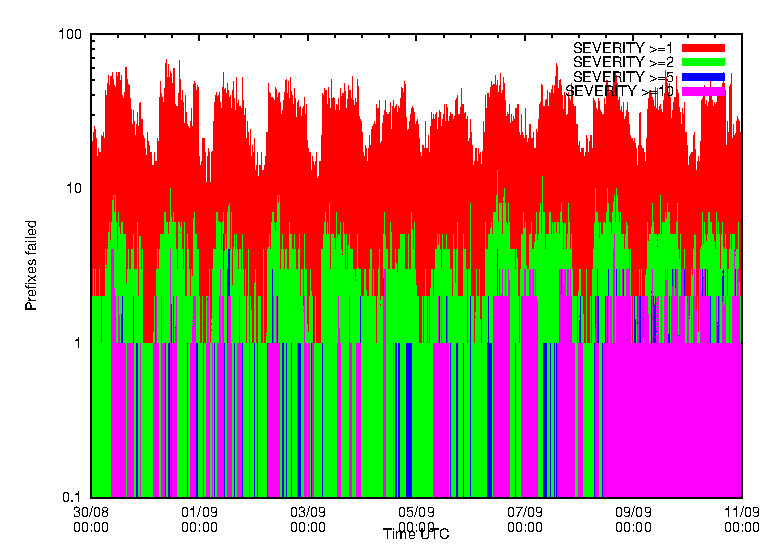
\includegraphics[width=9cm]{images/prefix_failed_ipv4.eps}
\caption{Traffic composition and volume of the three network telescopes. Source: Wustrow et al.}
\label{fig:Wustrow_spatial}
\end{figure}
The server socket detection and the ongoing monitoring thereof are already implemented. A one-week long netflow data trace of november 2010 was used to test this implementation. Therefore, some interesting statistical properties of the server sockets can already be shown.


% %%%%%%%%%%%%%%%%%%%%%%%%%%%%%%%%%%%%%%%%%%%%%%%%%%%%%%%%%%%%%%%
\bibliographystyle{abbrv} 
%\bibliographystyle{apalike} 
\bibliography{95_bib}
\end{document}
